% !TEX program = ptex2pdf -l -ot "-kanji=utf8 -synctex=1"←こっちの環境で動かせるようにしてるだけだから気にしないで！

% --- pLaTeX用に書き換えたテンプレート ---
\documentclass[dvipdfmx, a4paper, 10pt]{jsarticle} % pLaTeX用の標準クラス
\usepackage[margin=25mm]{geometry} % 余白設定（これ1行で上下左右の余白を美しく設定できる）
\usepackage[dvipdfmx]{graphicx} % 画像を扱うためのパッケージ（pLaTeXならdvipdfmxの指定が必須！）
\usepackage{url} % 文中にURLを簡単に表示させる
\usepackage{amsmath} % 高度な数式や複雑な式のレイアウトを可能にする
\usepackage{latexsym} % 数学記号や特別な文字を使うことを考慮して追加
\usepackage{float} % 図や表の配置を指定する（[H]を使うため）

% ==========================================
% 【LaTeXを書く時の絶対ルール】
% 1. 「\」や「スペース」は必ず半角入力！全角スペースはエラーの最大の原因！
% 2. 「%」の後ろに書いた文字はコメントになる（PDFには表示されず、メモに使える）
% 3. 「$, &, _, {, }」などの記号は特別な意味を持つため、
%    そのまま画面に出したい時は前に「\」をつけること（例: \$）
% 4. \begin{...} と \end{...} は絶対にペアで使うこと！
% 5. 文章の改行に「\\」は使わない！段落を変える時は「1行の空行（エンター2回）」を入れること。
% ==========================================

\begin{document}

\begin{center} % タイトルの部分
  {\huge \textbf{実験題目}} \\[1em] % \\[1em] で少しだけ広めの改行幅を取る
  {\large \textbf{電気通信大学情報理工学域I\hspace{-1.2pt}I\hspace{-1.2pt}I類}} \\ % ⅡやⅢを出力しようとするとエラーが出るのでIを並べて無理やり出力する
  {\large \textbf{学籍番号: 26xxxxx \quad 名前: xxxx}} \\[1em] % \quad は空白を入れるコマンド
  {\textbf{\today\ 作成}} % \today でビルドした日の日付が自動的に入る
\end{center}

\section{目的}

% ここに目的を書く

\section{原理}

% ここに原理を書く

% 数式の書き方 -----------------------------------
\begin{equation} % 数式を書くときは equation 環境を使う
  y = \frac{x}{3} \times a % 分数は \frac、掛け算記号は \times
  \label{eq:keisan} % 数式を参照するためのラベル
\end{equation}

式\eqref{eq:keisan}より～ % ← 数式はこれで参照すると自動でカッコがつく

\begin{equation*}
  \lambda = \frac{c}{\nu} % ギリシャ文字は英語で入力するといい感じになる
\end{equation*} % 式番号を消したいときは*をつける
% ------------------------------------------------

$\lambda = 1.5 \times 10^{-10} \, \mathrm{m}$ 
% 文章中に数式を書くときは$で囲む。単位は斜体にしてはいけないので \mathrm{} で囲むこと。
% 数値と単位の間にはスペースを入れる（\, を入れると綺麗な間隔になる）


\section{方法}

\subsection{〇〇〇の方法}
% ここに方法を書く

\subsection{△△△の方法}
% ここに方法を書く
% 一つの節に収まらない場合は subsection を使うといい


\section{結果}

% 画像の貼り方 -----------------------------------------
% 注意: 画像ファイルはtexファイルと同じフォルダ（同じ場所）に入れること！！！！
\begin{figure}[H] % Hをつけるとここに強制的に配置されるわ。まずはこれを使うと安心
  \centering
  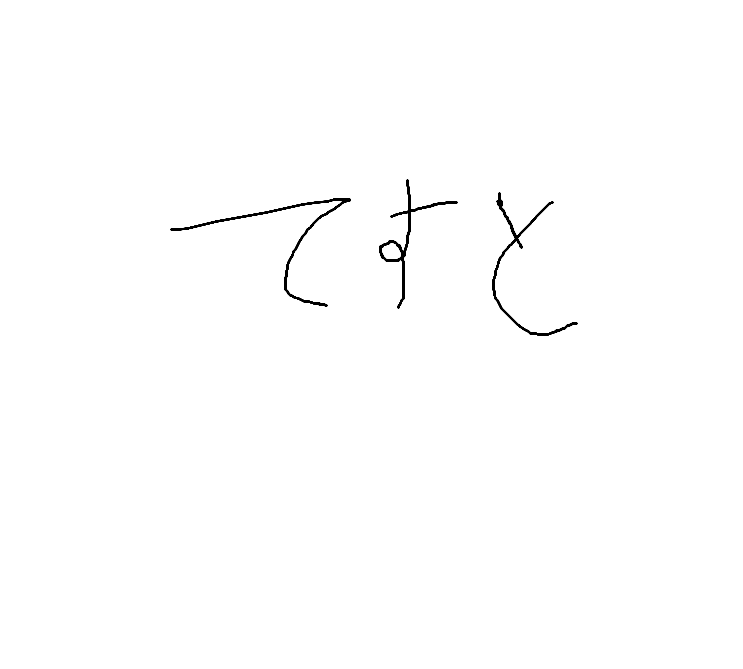
\includegraphics[width=10cm]{ファイル名.png} % widthで幅を指定。拡張子（.以降）までしっかり書くこと
  \caption{図の説明} % キャプションを書く。説明がいらないなら消してもよい
  \label{fig:ラベル} % 図を参照するときに使うラベル
\end{figure}
% --------------------------------------------------------

図\ref{fig:ラベル}より～ % 図を参照するときは \ref を使う

% 表の貼り方 -------------------------------------------------
\begin{table}[H]
  \centering
  \caption{表の説明} 
  \begin{tabular}{cccc} % cの数は表の列の数に合わせる(cは中央寄せ、lは左、rは右)。今回は4列
    & 要素1 & 要素2 & 要素3 \\ \hline % \hline で横線を引く、&は列の区切り、\\は行の区切り
    要素4 & & & \\
    & & 要素5 & \\ \hline
  \end{tabular}
  \label{tab:ラベル} 
\end{table}
% --------------------------------------------------------

表\ref{tab:ラベル}より～

% 学習用おすすめサイト: https://guides.lib.kyushu-u.ac.jp/LaTeX-LectureNote/equations
% わからなかったらGeminiなどの生成AIに聞くのも手！


\section{考察}

% ここに考察を書く


\begin{thebibliography}{99} % 参考文献を書くところ
% 参考文献の書き方はちゃんと調べること
% (おすすめサイト: https://www.lib.niigata-u.ac.jp/wp-content/uploads/2023/10/reference2022.pdf)
\bibitem{ref:label1} 著者名『本のタイトル』出版社、発行年。
\bibitem{ref:label2} 著者名「論文のタイトル」『雑誌名』巻号、ページ、発行年。
\end{thebibliography}

\end{document}